\chapter{Appendix B --- Data Sets}\label{ch:appendixB}

The images used for the evaluation in \autoref{ch:evaluation} can be found here.
The captions relate the images to their position in the bird's eye view from
that chapter.

\section{Train Station Data Set}
\FloatBarrier
\begin{figure}[h]
   \begin{subfigure}[t]{.33\textwidth}
      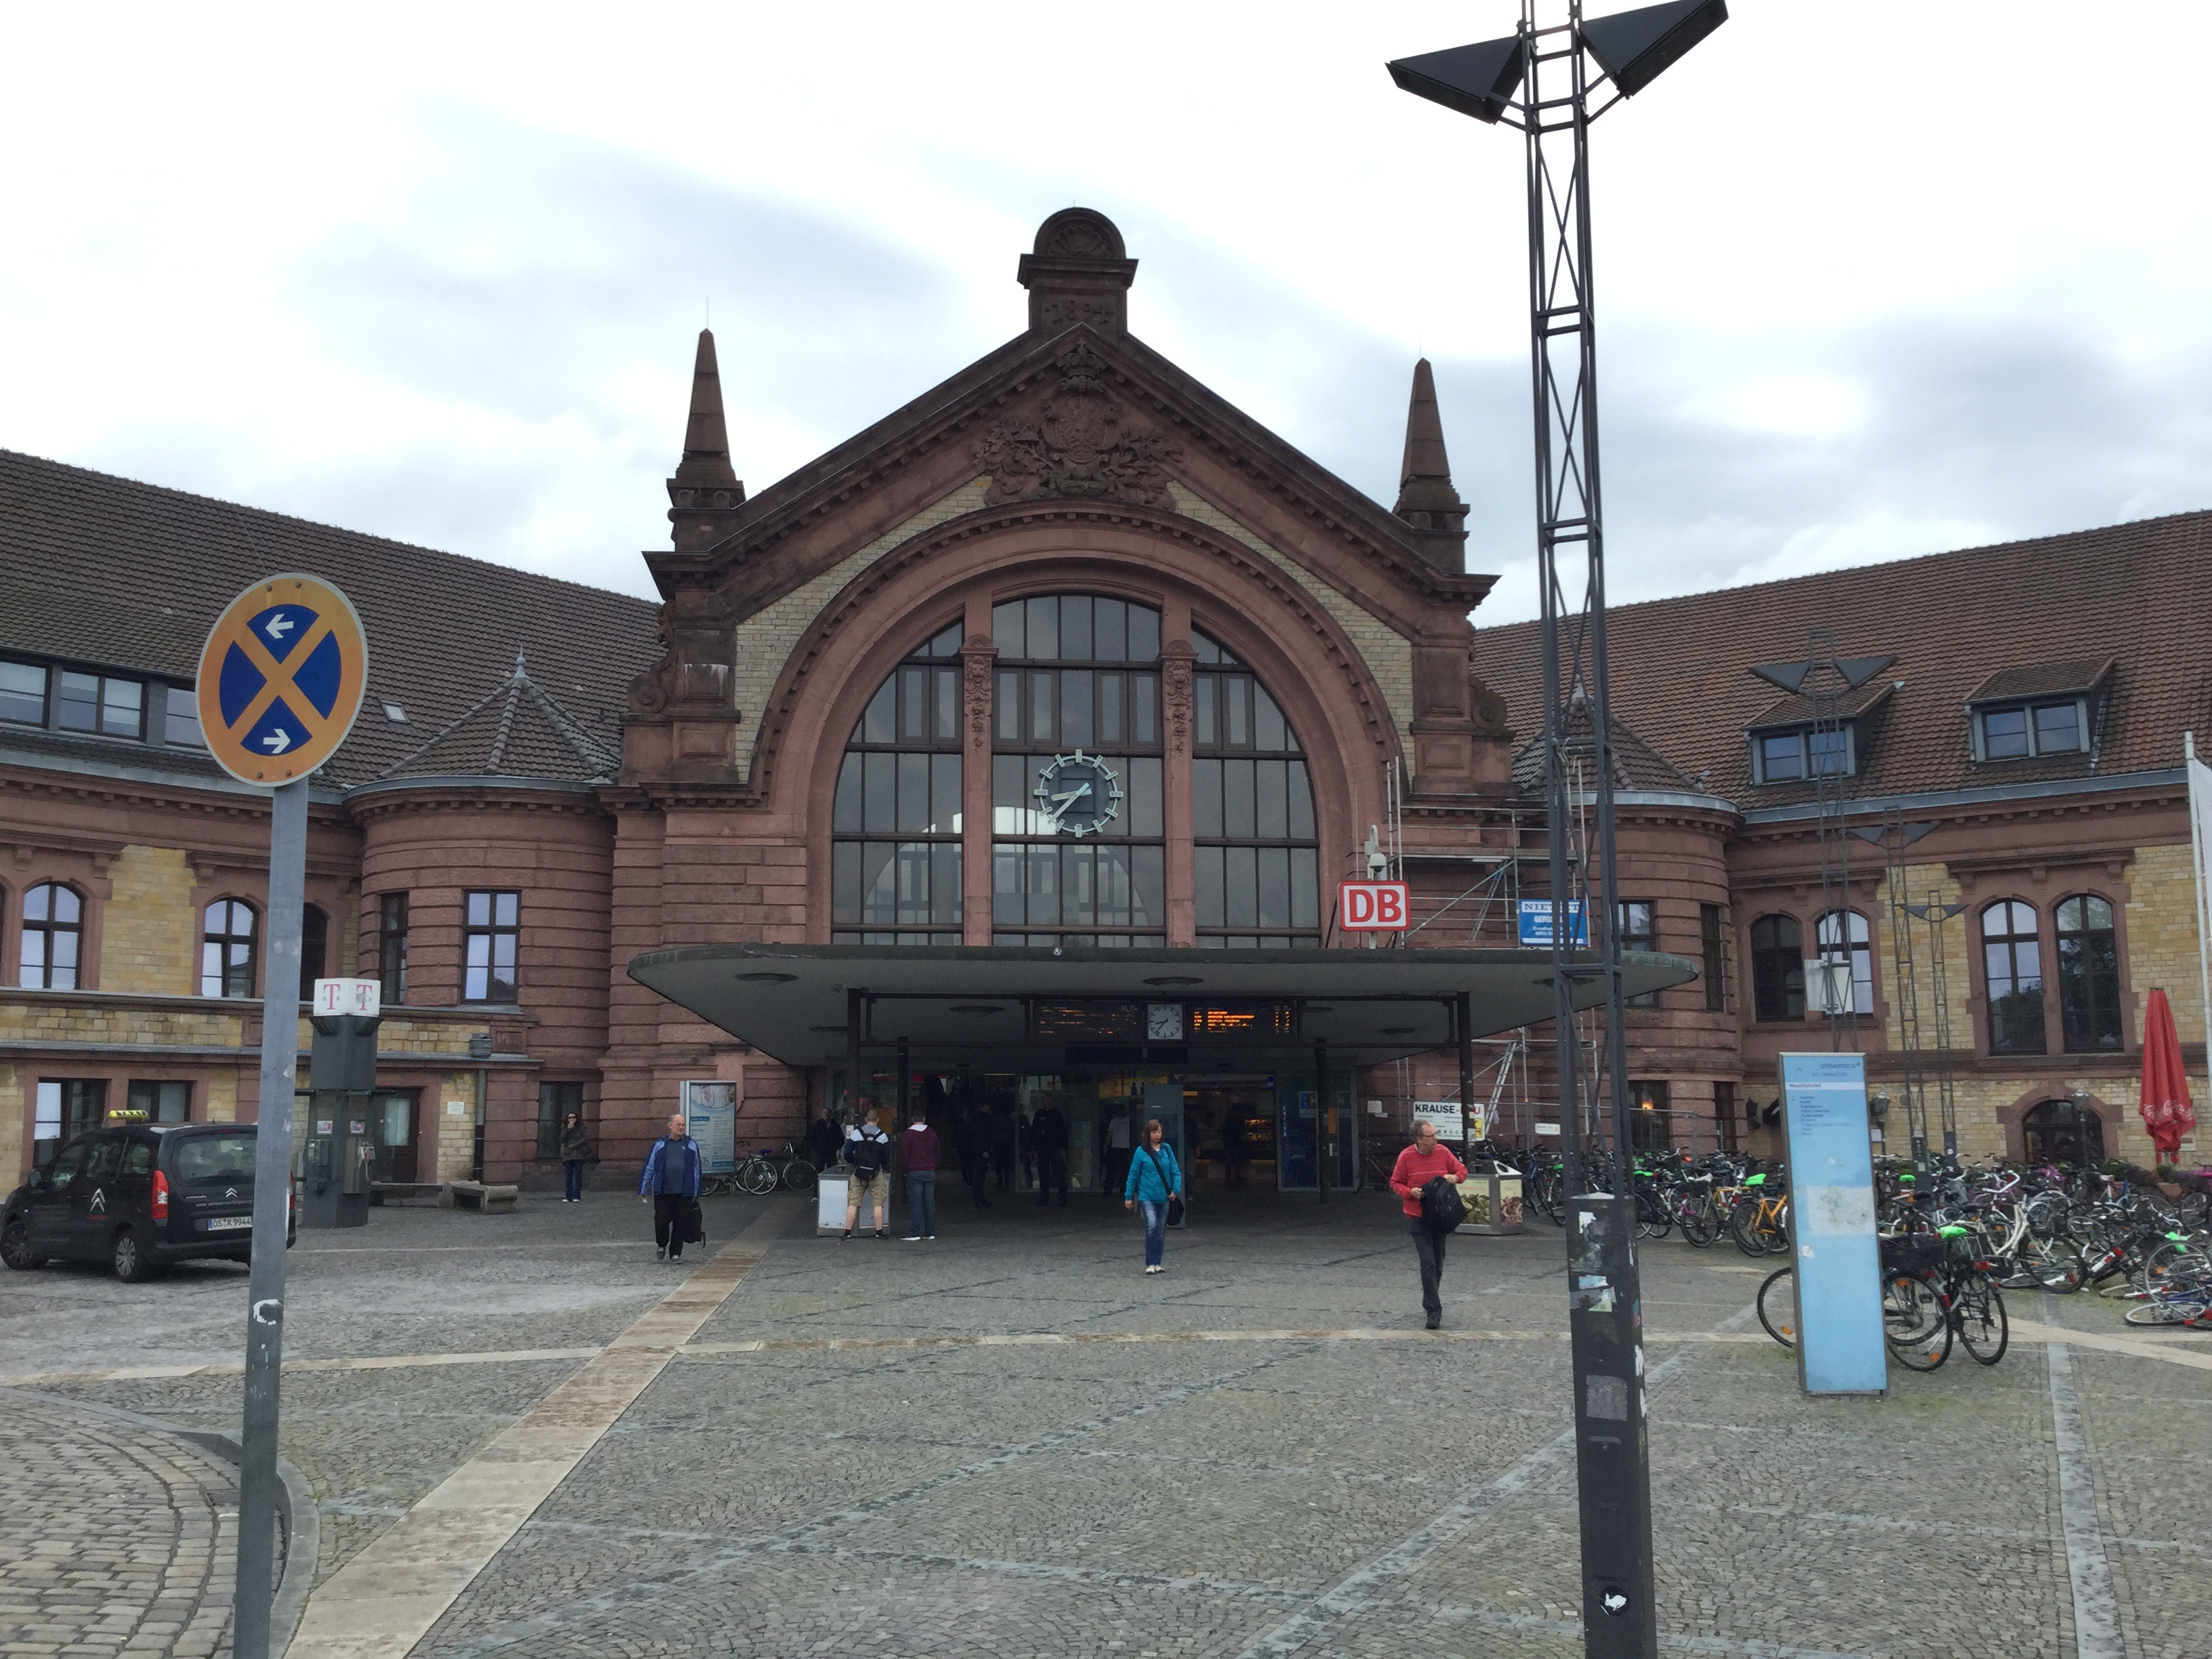
\includegraphics[width=\textwidth]{gfx/bahnhof_imgs/0.JPG}
      \caption{$0$: The ``reference'' image}
   \end{subfigure}
   \begin{subfigure}[t]{.33\textwidth}
      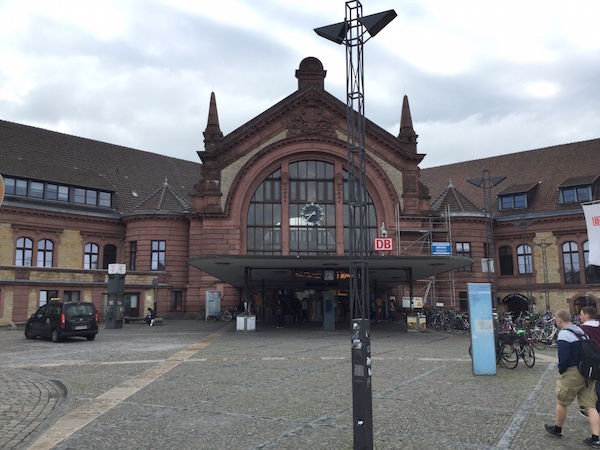
\includegraphics[width=\textwidth]{gfx/bahnhof_imgs/5.JPG}
      \caption{$4$}
   \end{subfigure}
   \begin{subfigure}[t]{.33\textwidth}
      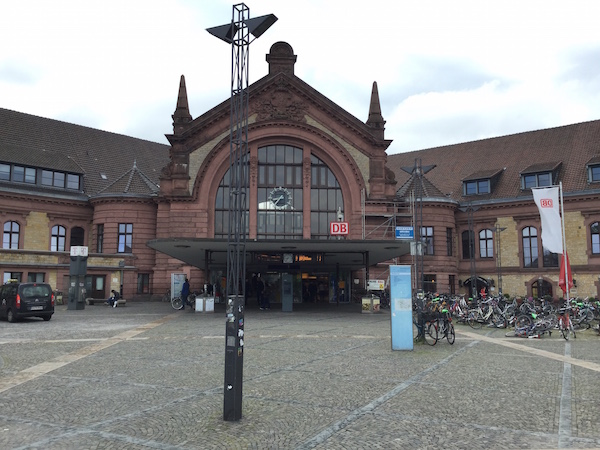
\includegraphics[width=\textwidth]{gfx/bahnhof_imgs/4.JPG}
      \caption{$3$}
   \end{subfigure}

   \begin{subfigure}{.33\textwidth}
      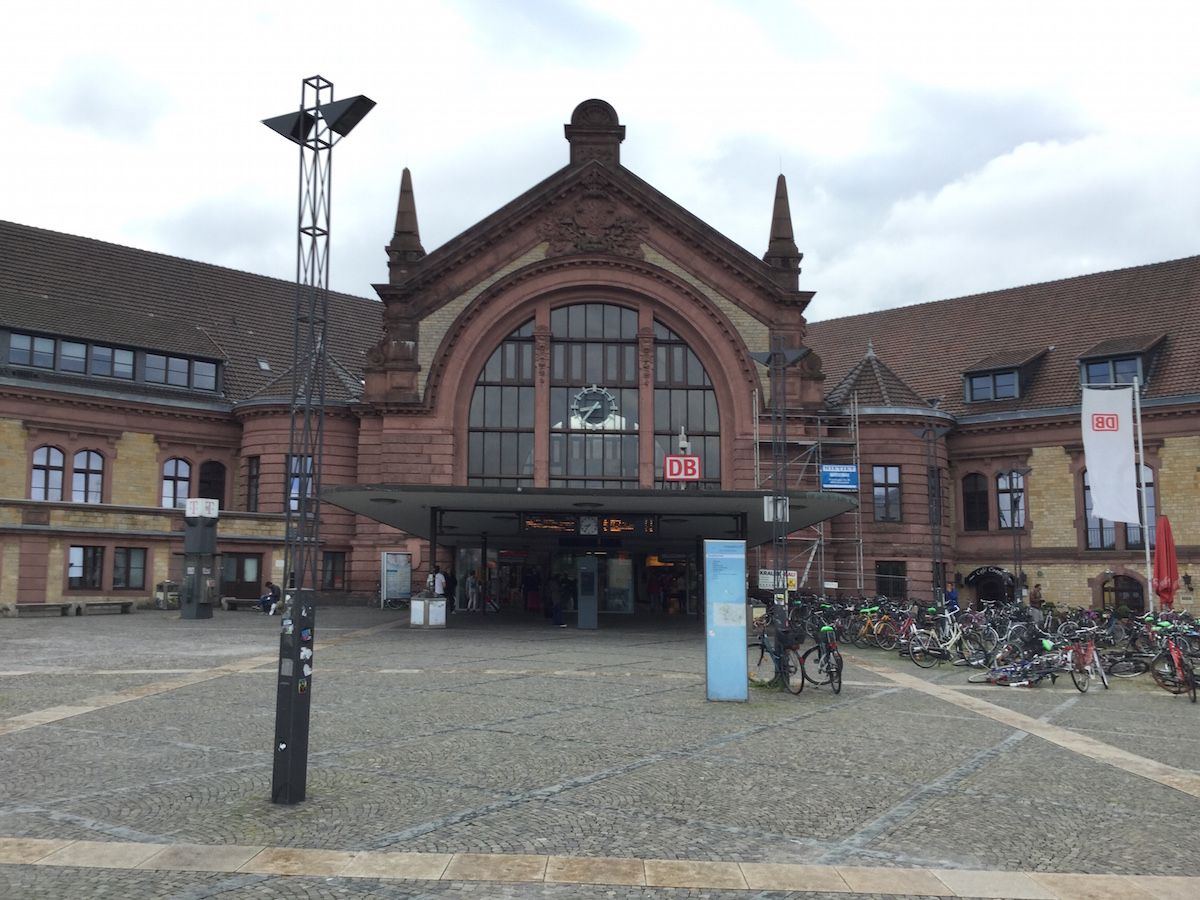
\includegraphics[width=\textwidth]{gfx/bahnhof_imgs/3.JPG}
      \caption{$2$}
   \end{subfigure}
   \begin{subfigure}{.33\textwidth}
      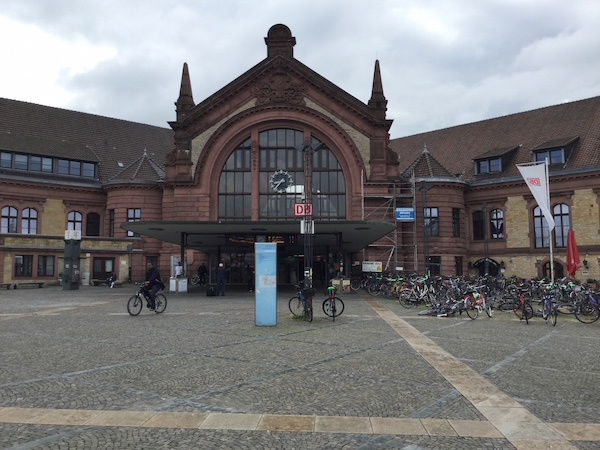
\includegraphics[width=\textwidth]{gfx/bahnhof_imgs/2.JPG}
      \caption{$1$}
   \end{subfigure}
   \begin{subfigure}{.33\textwidth}
      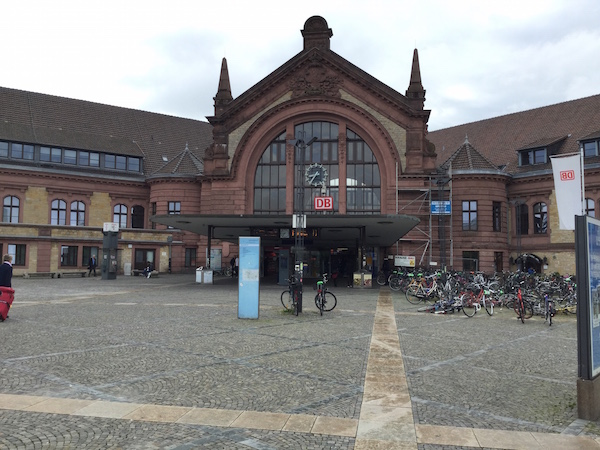
\includegraphics[width=\textwidth]{gfx/bahnhof_imgs/1.JPG}
      \caption{First frame}
   \end{subfigure}
   \caption[Train station images]{Images in the train station data set}
   \label{fig:train_imgs}
\end{figure}
\FloatBarrier

\newpage
\section{Manor Data Set}
\FloatBarrier
\begin{figure}[h]
   \begin{subfigure}[t]{.33\textwidth}
      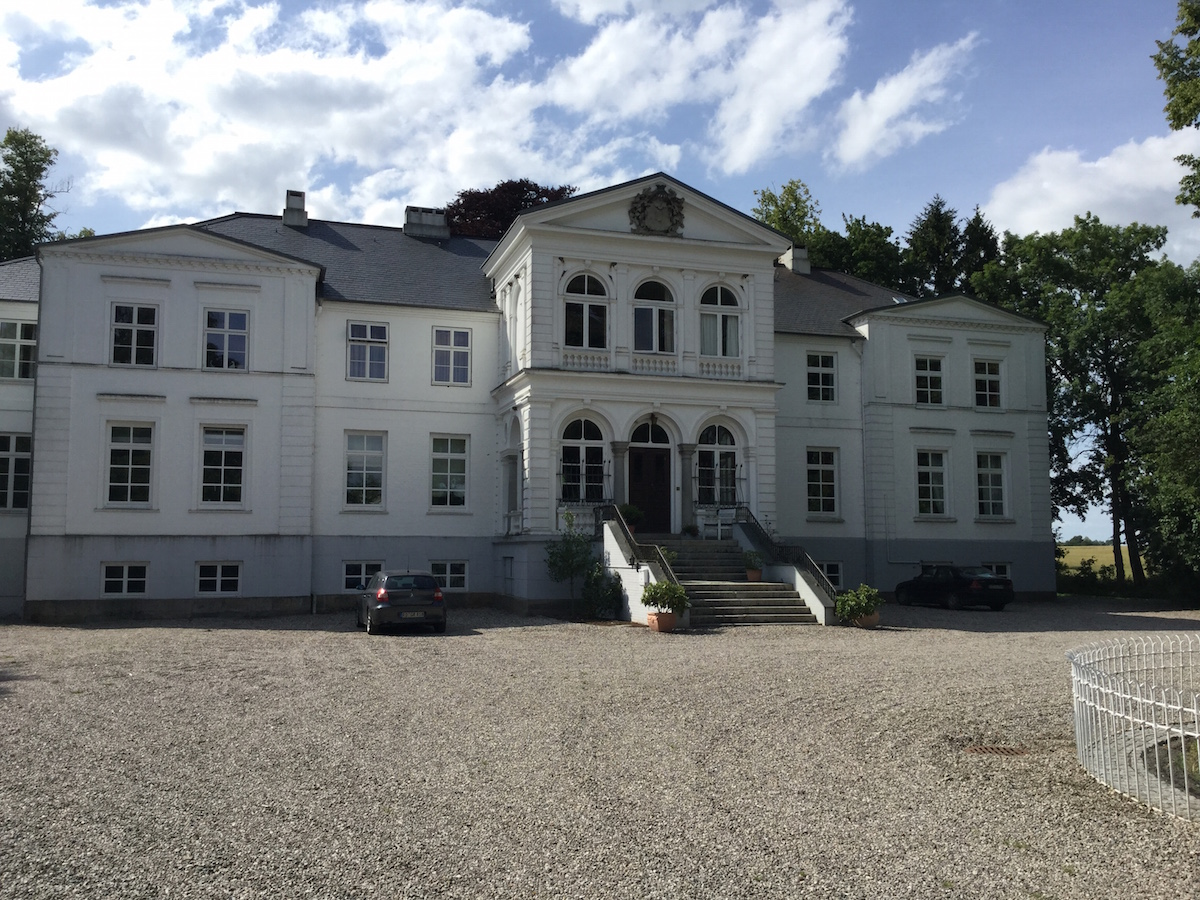
\includegraphics[width=\textwidth]{gfx/manor_imgs/0_ref.JPG}
      \caption{$0$: The ``reference'' image}
   \end{subfigure}
   \begin{subfigure}[t]{.33\textwidth}
      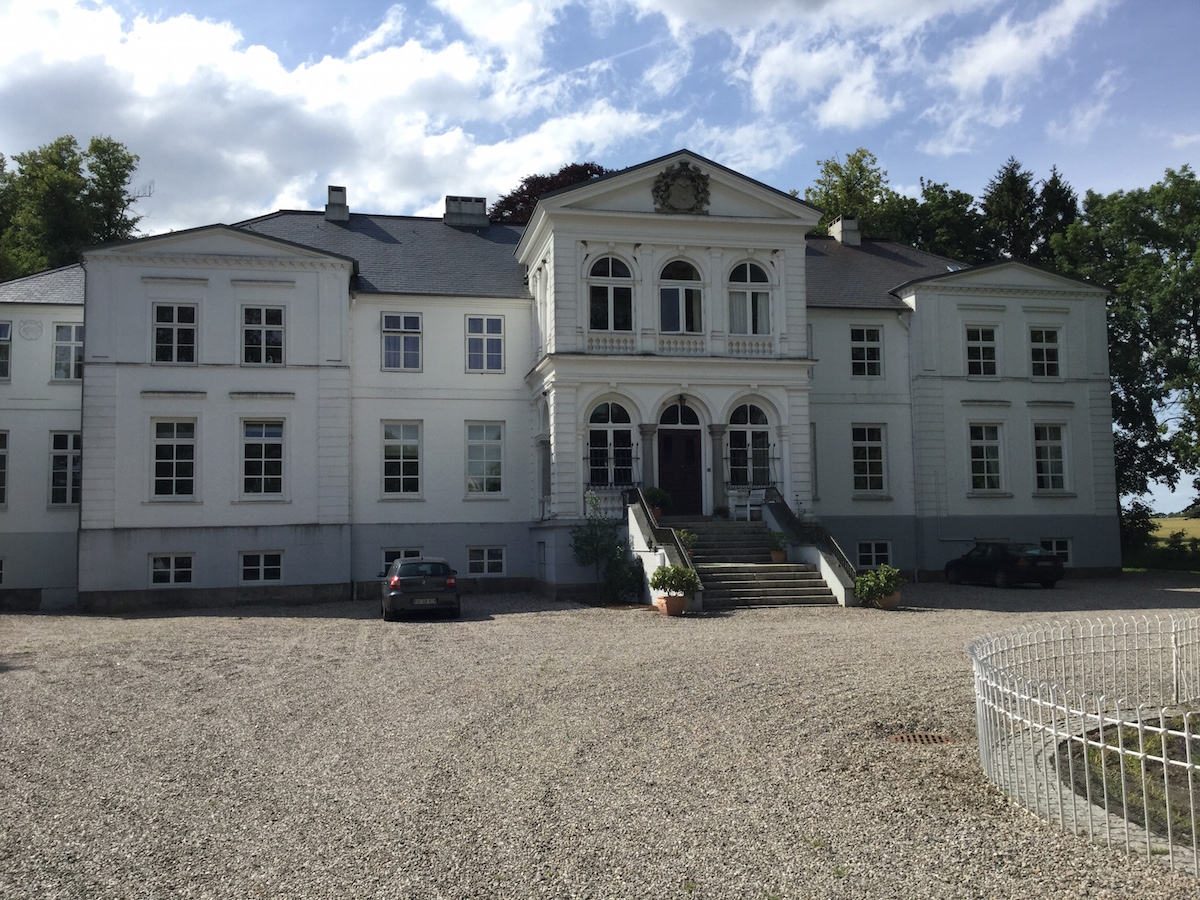
\includegraphics[width=\textwidth]{gfx/manor_imgs/1.JPG}
      \caption{$1$}
   \end{subfigure}
   \begin{subfigure}[t]{.33\textwidth}
      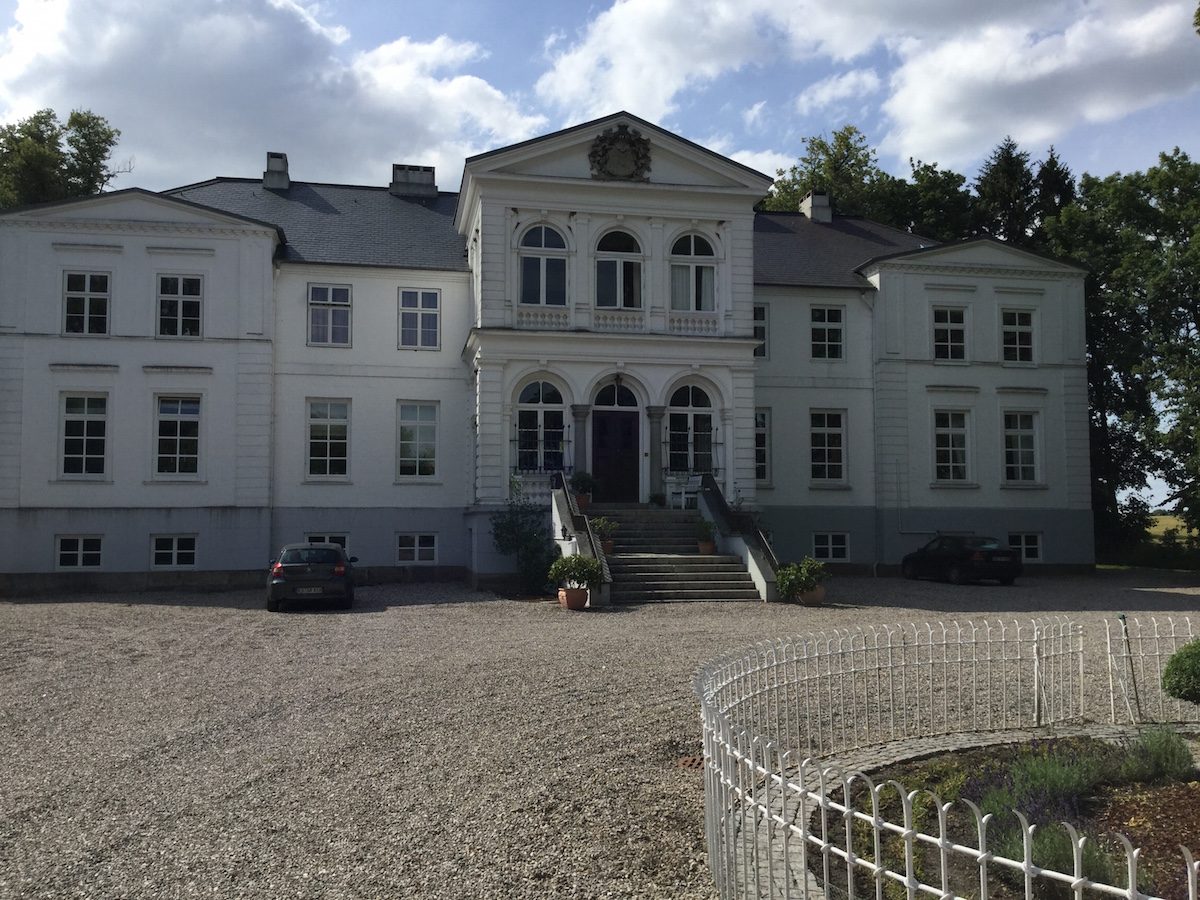
\includegraphics[width=\textwidth]{gfx/manor_imgs/2.JPG}
      \caption{$2$}
   \end{subfigure}

   \begin{subfigure}{.33\textwidth}
      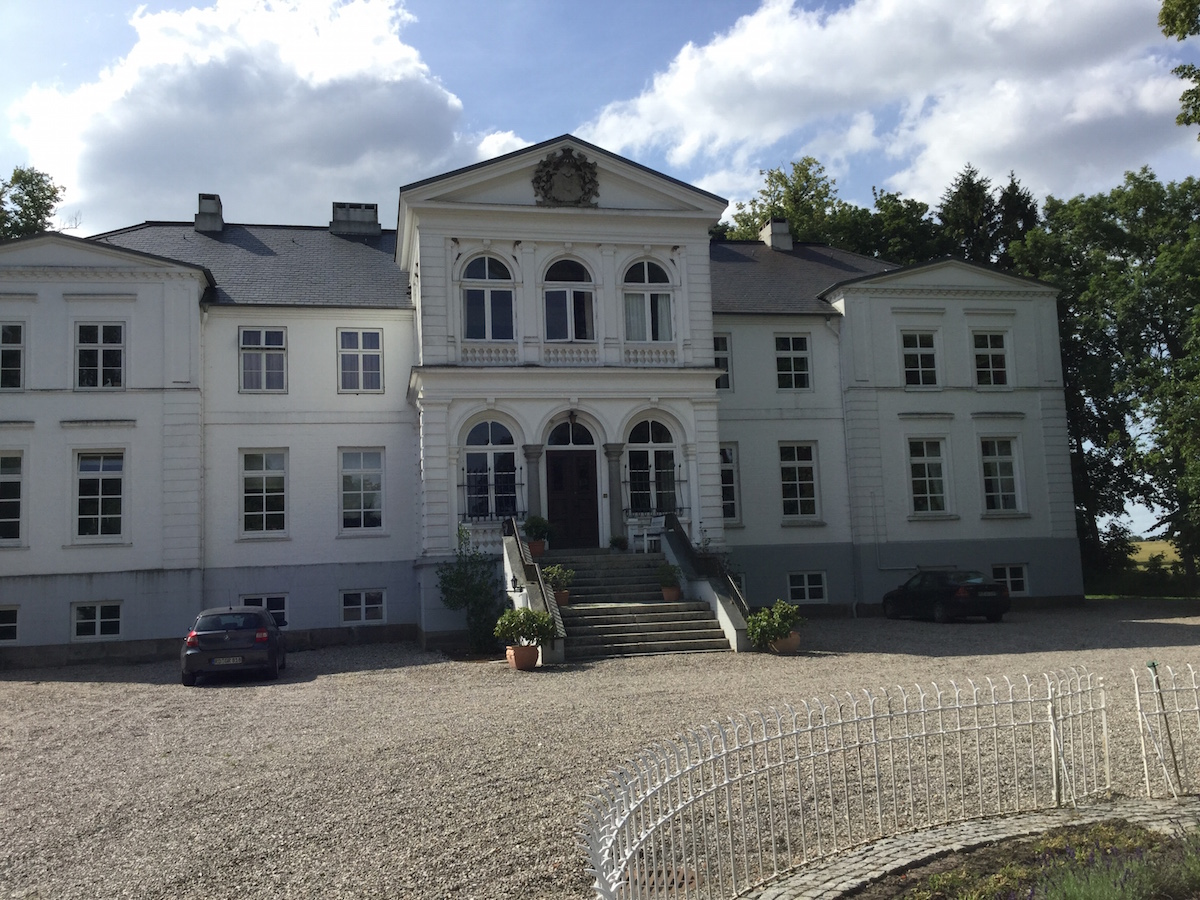
\includegraphics[width=\textwidth]{gfx/manor_imgs/3.JPG}
      \caption{$3$}
   \end{subfigure}
   \begin{subfigure}{.33\textwidth}
      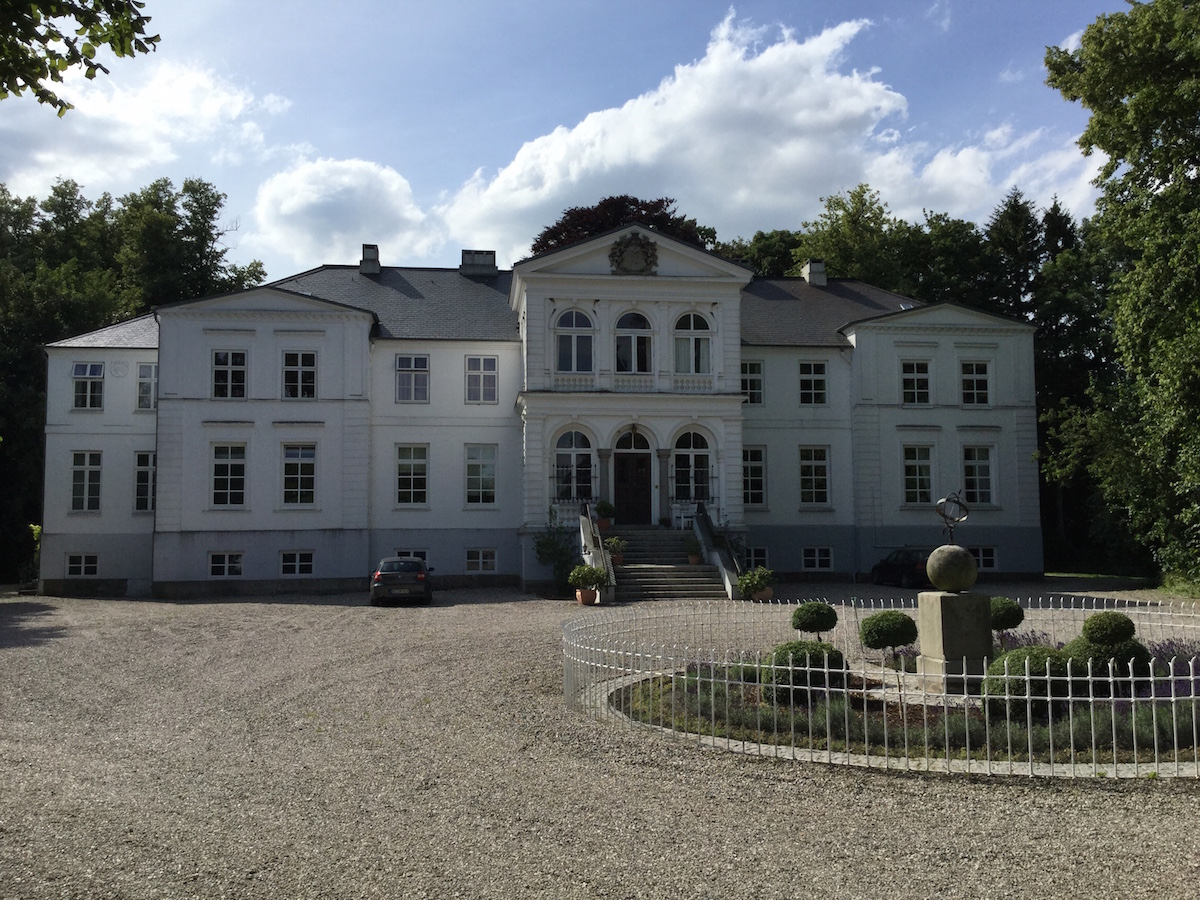
\includegraphics[width=\textwidth]{gfx/manor_imgs/4.JPG}
      \caption{$4$}
   \end{subfigure}
   \begin{subfigure}{.33\textwidth}
      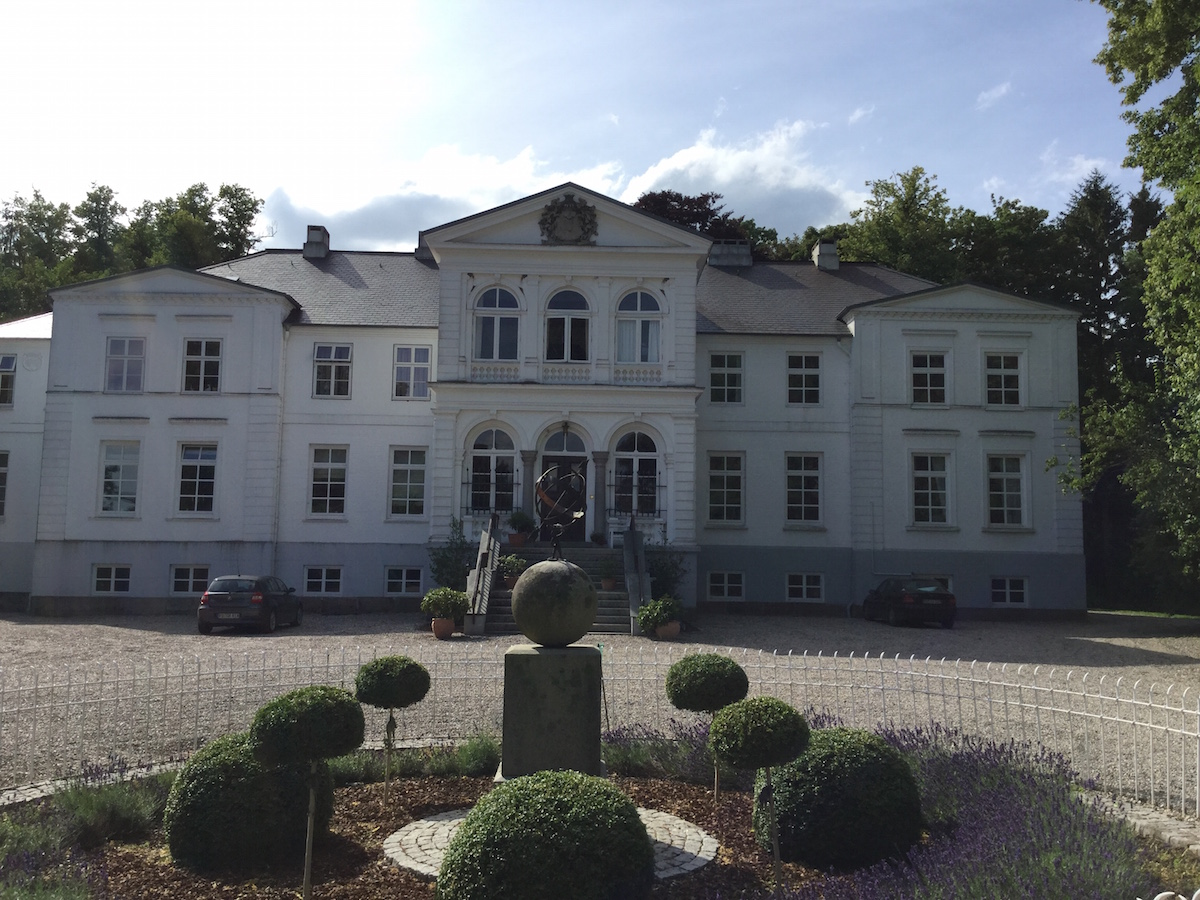
\includegraphics[width=\textwidth]{gfx/manor_imgs/5.JPG}
      \caption{$5$}
   \end{subfigure}

   \begin{subfigure}{.33\textwidth}
      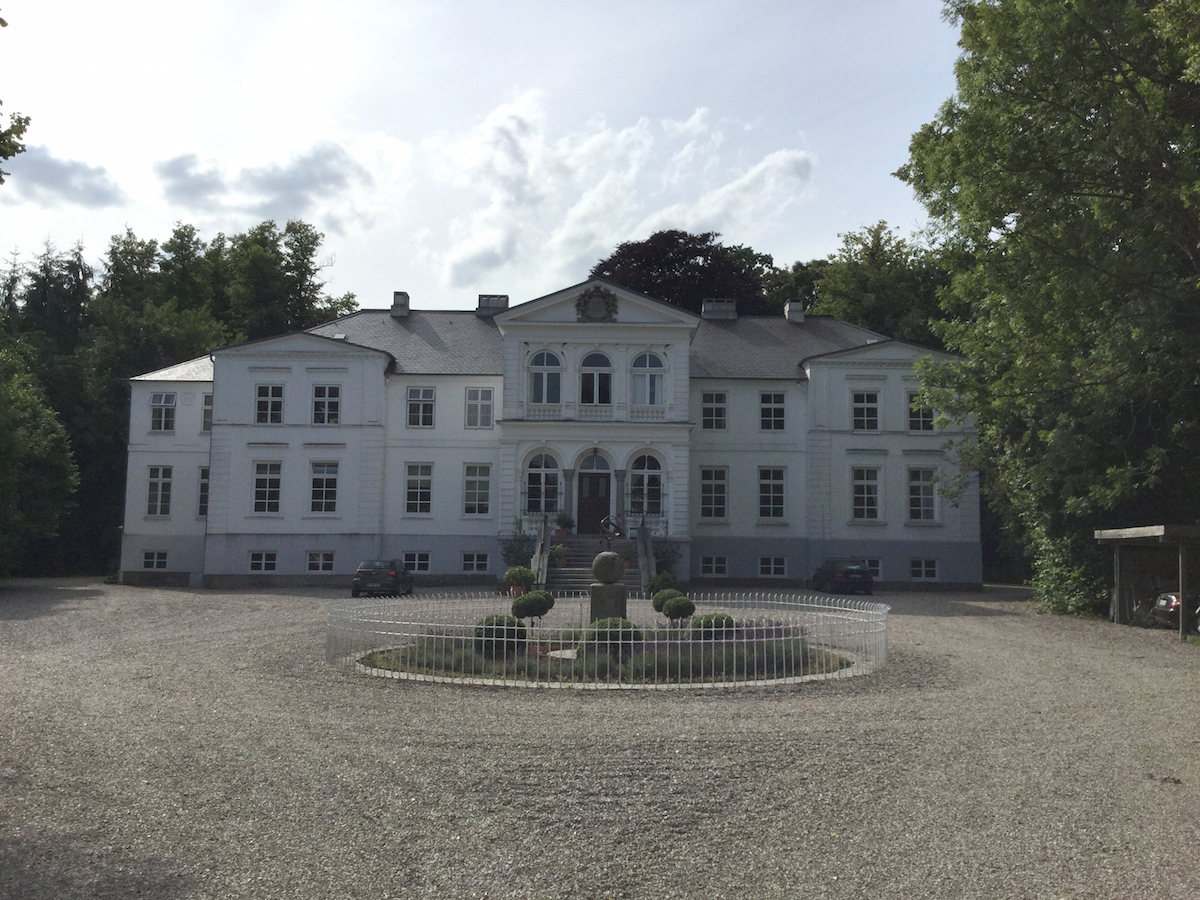
\includegraphics[width=\textwidth]{gfx/manor_imgs/9.JPG}
      \caption{$6$}
   \end{subfigure}
   \begin{subfigure}{.33\textwidth}
      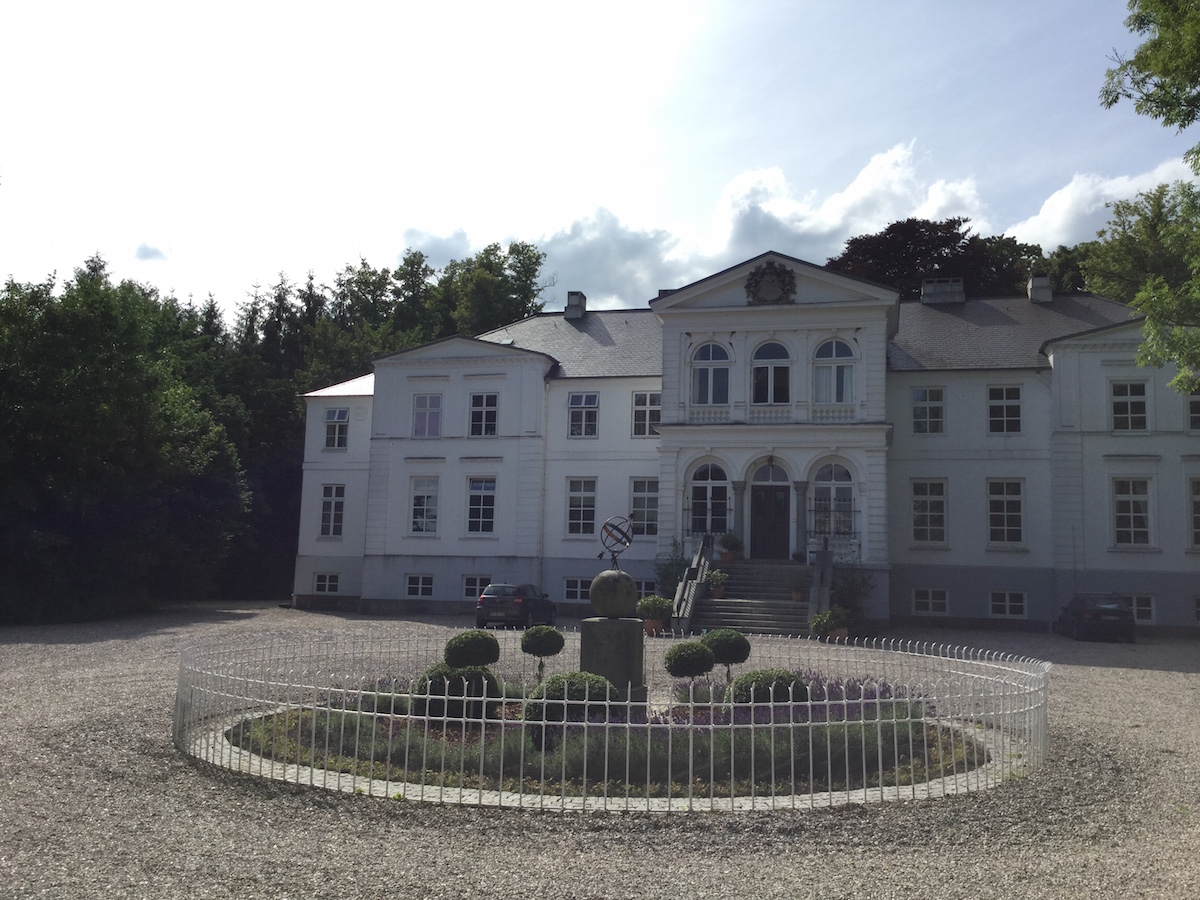
\includegraphics[width=\textwidth]{gfx/manor_imgs/first_frame_centered.JPG}
      \caption{First frame}
   \end{subfigure}
   \caption[Manor images]{Images in the manor data set}
   \label{fig:manor_imgs}
\end{figure}
\FloatBarrier

